\documentclass{ecai}

\usepackage{latexsym}
\usepackage{amssymb}
\usepackage{amsmath}
\usepackage{booktabs}
\usepackage{enumitem}
\usepackage{graphicx}
\usepackage{color}
\usepackage{tikz}
\usetikzlibrary{arrows.meta,positioning,fit,backgrounds}

\newcommand{\BibTeX}{B\kern-.05em{\sc i\kern-.025em b}\kern-.08em\TeX}
\newcommand{\rupee}{INR\,}

\begin{document}

\begin{frontmatter}

\paperid{1}

\title{TripGraph AI: A Grounded Multi-Agent System for \\
Conversational Group Travel Itinerary Planning}

\author[A]{\fnms{Ujjwal}~\snm{Rattan}\thanks{Corresponding Author. Email: ujjwalrattan@iisc.ac.in.}}
\author[A]{\fnms{Naveen}~\snm{Venturi}}
\author[A]{\fnms{Navneet}~\snm{Samra}}
\author[A]{\fnms{Siddaraju}~\snm{D.H.}}

\address[A]{Indian Institute of Science, Bengaluru, India}

\begin{abstract}
Large language models can write plausible travel itineraries but routinely
hallucinate places, distances, opening hours and prices, and collapse on the
constraint arithmetic real trips demand. We present \emph{TripGraph AI}, a
deployed multi-agent system that converts free-form group chat into a
constraint-aware, day-by-day itinerary rendered on an interactive map. Rather
than a single generative call, TripGraph routes a twelve-node LangGraph
pipeline in which a curated knowledge graph supplies verified candidate places
and a battery of real APIs (routing, places, weather, rail) ground every
decision. A single \emph{Itinerary Architect} LLM call then \emph{selects,
sequences and clusters} activities per day over a real driving-time matrix,
emitting explicit inter-stop travel legs, fatigue pacing and per-event
reasoning. We further introduce \emph{per-role model routing}: reasoning-heavy
roles use a frontier model (Claude) while high-volume roles use a free,
fast model (Gemini Flash-Lite), cutting paid-model calls by ${\sim}75\%$ with
no quality regression. The system is live behind a domain with HTTPS. We
describe the architecture, a cost/latency analysis, robustness measures, and a
worked example; supporting detail is provided in numbered appendices.
\end{abstract}

\end{frontmatter}

\section{Introduction}
\label{sec:intro}

Planning a group trip is a constraint-satisfaction problem wrapped in a
conversation. A chat such as ``\emph{4 days in Goa from Chandigarh, around
\rupee40k each, beaches and seafood, flying, group of 4}'' implies a budget
envelope, a transport mode, a geography to sequence, opening hours to respect,
and a group whose energy must be paced. Asking a single large language model
(LLM) to emit the whole plan is attractive but fragile: models invent
attractions, misstate inter-city distances, assign impossible same-day
schedules, and silently violate the budget~\citep{xie2024travelplanner}.

Concretely, an end-to-end LLM exhibits four recurring failure modes on this
task: \emph{(i)} it hallucinates attractions or hotels that do not exist;
\emph{(ii)} it mis-estimates travel time and so over-packs days or assumes
teleportation between stops; \emph{(iii)} it loses the budget, quietly
returning plans that exceed the stated cap; and \emph{(iv)} it ignores soft
human factors such as cumulative fatigue. Each of these is a place where a
\emph{fact} or a \emph{computation}, not fluent text, is required.

TripGraph AI takes the opposite stance. The LLM is used where it is strong
--- selection, sequencing and natural-language reasoning --- while a curated
knowledge graph (KG) and live APIs own everything that must be \emph{true}:
which places exist, how far apart they are, what the weather will be, and what
things cost. This mirrors retrieval-augmented generation~\citep{lewis2020rag}
and tool-use agents~\citep{yao2023react,schick2023toolformer}, but is
specialised into a fixed, auditable pipeline rather than a free-running agent
loop, so that every plan is reproducible and every fact is attributable. The
fixed control flow is a deliberate trade: we give up the open-endedness of an
autonomous agent in exchange for predictable latency, bounded cost, and the
ability to point at the exact node responsible for any field in the output.

\paragraph{Contributions.}
\begin{enumerate}[leftmargin=1.4em,itemsep=1pt]
\item A deployed twelve-node \textbf{grounded planning pipeline}
(Section~\ref{sec:arch}) that fuses a curated KG with five external data
services; the full node roster is in Appendix~\ref{app:nodes}.
\item The \textbf{Itinerary Architect} (Section~\ref{sec:architect}): one
structured LLM pass that plans a multi-day trip over a real travel-time matrix
with explicit travel legs and fatigue pacing. A worked output is in
Appendix~\ref{app:example}.
\item \textbf{Per-role multi-LLM routing} (Section~\ref{sec:routing}): a
configuration-only mechanism that offloads ${\sim}75\%$ of LLM calls to a free
model while protecting quality; cost/latency data in Appendix~\ref{app:cost}.
\item A \textbf{robustness and deployment} story (Section~\ref{sec:deploy}):
prompt-injection guardrails (Appendix~\ref{app:guard}), graceful degradation,
and a one-command cloud deployment (Appendix~\ref{app:deploy}).
\end{enumerate}

\section{System architecture}
\label{sec:arch}

TripGraph is a FastAPI backend orchestrating a LangGraph~\citep{langgraph2024}
state graph, with a React/Vite map-centric frontend. A request flows through
the stages in Figure~\ref{fig:pipeline}. The chat is first parsed into a typed
\texttt{constraints} object; a validator checks for conflicts and fills safe
defaults. A two-pass retriever then assembles candidate routes, hotels,
activities and restaurants \emph{KG-first}, falling back to APIs only for gaps,
and caching results to disk. Independent grounding agents (flights, rail,
weather, web insights) run \emph{concurrently}. The Architect consumes all of
this and emits the plan, which is then enriched (place photos, road polylines),
scored for fatigue, and reviewed.

\begin{figure}[t]
\centering
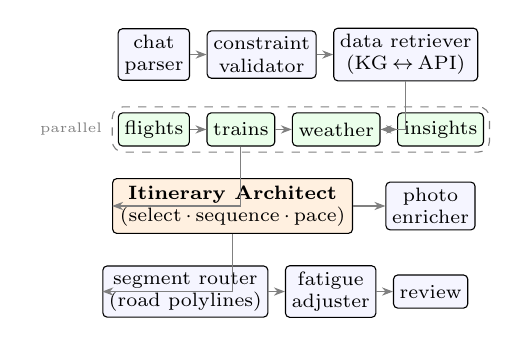
\begin{tikzpicture}[
  font=\scriptsize,
  node distance=2.1mm,
  box/.style={draw,rounded corners=1.5pt,align=center,inner sep=2.2pt,
              minimum height=4.2mm,fill=blue!4},
  arch/.style={draw,rounded corners=1.5pt,align=center,inner sep=2.6pt,
               minimum height=4.6mm,fill=orange!12},
  gnd/.style={draw,rounded corners=1.5pt,align=center,inner sep=2.2pt,
              minimum height=4.2mm,fill=green!8},
  ar/.style={-{Stealth[length=1.4mm]},gray}]
\node[box] (parse) {chat\\parser};
\node[box,right=of parse] (val) {constraint\\validator};
\node[box,right=of val] (ret) {data retriever\\(KG\,$\leftrightarrow$\,API)};
\node[gnd,below=4mm of parse] (fl) {flights};
\node[gnd,right=of fl] (tr) {trains};
\node[gnd,right=of tr] (we) {weather};
\node[gnd,right=of we] (ins) {insights};
\node[arch,below=4mm of fl,xshift=10mm] (arch) {\textbf{Itinerary Architect}\\(select\,$\cdot$\,sequence\,$\cdot$\,pace)};
\node[box,right=of arch,xshift=2mm] (photo) {photo\\enricher};
\node[box,below=4mm of arch,xshift=-6mm] (seg) {segment router\\(road polylines)};
\node[box,right=of seg] (fat) {fatigue\\adjuster};
\node[box,right=of fat] (rev) {review};
\draw[ar] (parse)--(val); \draw[ar] (val)--(ret);
\draw[ar] (ret.south) |- (we.east);
\draw[ar] (fl)--(tr); \draw[ar] (tr)--(we); \draw[ar] (we)--(ins);
\draw[ar] (tr.south) |- (arch.west);
\draw[ar] (arch)--(photo);
\draw[ar] (arch.south) |- (seg.west);
\draw[ar] (seg)--(fat); \draw[ar] (fat)--(rev);
\begin{scope}[on background layer]
\node[draw,dashed,gray,rounded corners,fit=(fl)(ins),inner sep=2pt,
      label={[gray,font=\tiny]left:\,parallel}] {};
\end{scope}
\end{tikzpicture}
\caption{The TripGraph pipeline. Blue: structural nodes; green: concurrent
grounding agents; orange: the reasoning core. Constraint extraction and
validation precede a KG-first retrieval; the Architect plans over grounded
candidates; downstream nodes enrich, pace and review.}
\label{fig:pipeline}
\end{figure}

\paragraph{Constraint extraction and validation.}
The parser maps free text to a typed record --- origin, destination, dates,
duration, group size, budget per person, hotel tier, transport preferences,
must-include activities and risk tolerance --- emitting \texttt{null} for
anything not stated rather than inventing it. The validator then performs
lightweight constraint reasoning: it detects conflicts (e.g.\ an
``expedition''-tier hotel against a sub-budget cap, or night-driving avoidance
on a long self-drive leg) and supplies safe defaults for non-critical fields,
recording each assumption so the user can review and override it before
planning proceeds. Only when the minimal fields are present does the graph
advance to retrieval.

\paragraph{Two-pass, KG-first retrieval.}
Retrieval runs in two passes. Pass one queries the knowledge graph for routes,
hotels, activities and restaurants matching the destination and tier. If
coverage is sufficient the system stops there; otherwise pass two calls
external services only for the missing slots and merges the results back, with
every fetched record written to a disk cache keyed by query so repeat trips are
near-instant. This ordering keeps the common case fast and free, reserves paid
API calls for genuine gaps, and bounds the blast radius of any single service
outage.

\paragraph{Knowledge graph as a guardrail.}
The KG is a curated store of $80{+}$ Indian destinations with activities,
hotels and transport options, each carrying coordinates, ratings, indicative
cost, fatigue/morale seeds and a confidence score. Crucially, the LLM never
invents a place: it \emph{chooses} from verified candidates, which is what
turns ``a plausible-sounding plan'' into ``a plan whose every stop exists''.
The KG also makes failure graceful --- if a live API is unavailable, the
cached/seed data still yields a coherent plan. The graph is queried through a
fallback layer (Neo4j when present, otherwise an equivalent JSON store), so the
system carries no hard database dependency and runs unchanged on a laptop or a
small cloud instance.

\section{The Itinerary Architect}
\label{sec:architect}

The Architect is the system's reasoning core and its main departure from
template-based planners. In a \emph{single} structured call it receives: the
constraints, the chosen transport mode and hotel, the candidate pool, a real
\emph{driving-time matrix} between the top candidates (from a routing API), the
day-by-day weather, and short web insights. It returns a JSON plan in which
each day is a sequence of typed events (activity, meal, travel, rest, hotel),
and every event carries a start time, duration, a one-line ``why'', a fatigue
and morale score, a skippability rating, and local tips.

Three design rules make the output usable rather than merely plausible.
\textbf{(i) Explicit travel legs:} the Architect inserts a \texttt{travel}
event between every pair of physical stops, with mode and a traffic buffer
computed from the matrix --- so the map shows city\,$\rightarrow$\,airport
road, flight, and airport\,$\rightarrow$\,hotel road, not teleportation.
\textbf{(ii) No idle gaps and realistic days:} each day begins at the hotel and
ends with a return leg, and post-arrival afternoons are filled with low-fatigue
activities rather than left blank. \textbf{(iii) Bounded density:} a hard cap
of seven events per day (enforced both in-prompt and by a post-processor that
trims only low-priority, non-essential stops) keeps plans readable and bounds
output length, which is the dominant latency term (Appendix~\ref{app:cost}).

\paragraph{Grounding the schedule in real travel time.}
The candidate set is too large to reason over pairwise in prose, so we first
compute a driving-time matrix $D \in \mathbb{R}^{n\times n}$ over the top-$n$
candidates (hotel included) from a routing API, and pass it to the Architect as
structured context. The model is instructed to minimise backtracking by
keeping consecutive same-day stops geographically close, using $D$ rather than
straight-line distance, and to size each travel leg's duration as the matrix
value plus a traffic buffer. This is where most LLM planners fail silently ---
they assume teleportation between stops --- and where a cheap matrix gives the
model the one signal it cannot estimate reliably on its own.

\paragraph{Pacing model.}
Each event $e$ receives base fatigue and morale seeds from the catalogue, which
the \emph{fatigue\_adjuster} then refines for context. Conceptually the
adjusted fatigue of the $k$-th event on a day is
%
\begin{equation}\label{eq:fatigue}
\hat{f}_k \;=\; \mathrm{clip}_{[0,10]}\!\Big( f^{\,0}_k
 + \alpha\, c_k + \beta\, \mathbb{1}[\text{rain}_k]
 + \gamma \!\!\sum_{j<k}\!\mathbb{1}[f^{\,0}_j \!\ge\! \tau] \Big),
\end{equation}
%
where $f^{0}_k$ is the seed, $c_k$ the cumulative distance travelled so far that
day, the indicator terms add load for adverse weather and for preceding
high-intensity stops, and $\alpha,\beta,\gamma,\tau$ are small fixed weights.
A symmetric rule lowers morale for repeated activity types. The resulting
$(\hat f, \hat m)$ pair drives the per-event \emph{skippability} rating the UI
uses to mark which stops are essential versus cuttable when a group is tired.

\paragraph{Self-critique.}
The Architect's plan is passed to a review agent that checks budget adherence,
constraint satisfaction and obvious infeasibility, and either approves it or
returns structured feedback for one bounded re-plan. The review verdict is
surfaced to the user as an advisory (e.g.\ a flagged budget overage) rather
than silently mutating the plan, keeping the system honest about its own
limitations.

\paragraph{Robust decoding.}
Because LLMs frequently wrap JSON in markdown fences and append trailing prose,
we parse with a tolerant decoder that strips fences and extracts the first
valid JSON value; this single fix eliminated a class of silent
fall-backs-to-template that we observed when migrating model families
(Appendix~\ref{app:guard}).

\section{Cost-aware multi-LLM routing}
\label{sec:routing}

A planning run issues many LLM calls of very different value: parsing and
validation are cheap and forgiving, whereas the Architect and the final review
demand strong structured reasoning. We exploit this with \emph{per-role
routing}: every agent calls \texttt{get\_llm(role)}, and the provider/model for
each role is resolved from environment variables, so any agent can be moved
between providers with no code change. Our deployed configuration (Table~\ref{tab:routing}) keeps the
Architect and Review on a frontier model (Claude) and routes the remaining
roles to a free, fast model (Gemini Flash-Lite). This cut paid-model calls per
plan from ${\sim}8$ to ${\sim}2$ ($\approx 75\%$ reduction) while preserving
itinerary quality, because the offloaded roles emit small, well-specified JSON
that the smaller model handles reliably given our tolerant decoder. Independent
roles (flights/trains, weather/insights) additionally execute in parallel
threads, overlapping their network latency. A full latency and cost breakdown
is given in Appendix~\ref{app:cost}.

\begin{table}[h]
\caption{Per-role model routing (deployed configuration).}
\label{tab:routing}
\centering
\begin{tabular}{lll}
\toprule
Role(s) & Model & Rationale \\
\midrule
Architect & Claude (frontier) & hardest reasoning \\
Review & Claude (frontier) & quality gate \\
Parser, validator & Gemini Flash-Lite & small, forgiving JSON \\
Flights, trains, fatigue & Gemini Flash-Lite & high volume \\
Explainer, enricher & Gemini Flash-Lite & narrative/lookup \\
\bottomrule
\end{tabular}
\end{table}

The mechanism is configuration-only: a global default plus
\texttt{LLM\_PROVIDER\_<ROLE>} / \texttt{LLM\_MODEL\_<ROLE>} overrides resolved
at call time. Swapping any agent between providers --- or onto a local model
for offline use --- requires editing environment variables, not code, which
made the cost optimisation a deployment decision rather than a code change.

\section{Map-native interface}
\label{sec:ui}

A plan is only as useful as its presentation, and a list of bullet points hides
exactly the spatial reasoning travellers care about. TripGraph therefore makes
the map the primary surface: the itinerary \emph{is} the map. Each stop is a
numbered pin in visiting order; consecutive stops are joined by the
\emph{actual} road polyline returned by the routing API, while inter-city legs
render as a dashed flight/rail arc, so a user immediately sees the
city-centre\,$\rightarrow$\,airport drive, the flight, and the
airport\,$\rightarrow$\,hotel drive rather than an implausible straight line.

Selecting a pin opens a detail popover anchored to that point in screen space
(it tracks the pin as the map pans and zooms), showing a live place photo and
rating fetched from the places API, the Architect's one-line ``why'', opening
hours, the fatigue/morale gauges from Equation~(\ref{eq:fatigue}), and local
tips. A per-day strip and a calendar-style timeline give the temporal view;
clicking a day flies the map to that day's bounding box and filters the
timeline, and clicking a timeline event highlights its pin --- the spatial and
temporal views are bidirectionally linked. A cost ledger breaks the budget into
transport, hotel (per night $\times$ nights), activities, food and
miscellaneous, so the user can see \emph{where} the money goes, not just the
total. Finally, a delay simulator lets the user inject a disruption; the
\emph{replanner} shifts, shortens or drops events to absorb it and explains in
plain language what changed and whether the return deadline still holds.

\section{Robustness and deployment}
\label{sec:deploy}

\paragraph{Degradation and safety.} Every external call is wrapped so that a
failure downgrades gracefully (e.g.\ missing polylines fall back to straight
segments; a rate-limited agent is skipped) rather than failing the plan. Chat
input passes a dual-layer prompt-injection guardrail
(Appendix~\ref{app:guard}). LLM timeouts and client/proxy read-timeouts were
tuned to exceed worst-case plan latency after we traced a ``default data''
symptom to a 120\,s cap firing mid-generation.

\paragraph{Deployment.} The system runs in production behind a domain with
Let's Encrypt HTTPS: an \texttt{nginx} reverse proxy serves the built SPA and
proxies the API to a \texttt{systemd}-managed backend; one script provisions
the whole stack (Appendix~\ref{app:deploy}). A private-preview gate lets the
site stay publicly visible while disabling credit-spending endpoints.

\section{Related work and conclusion}
\label{sec:related}

TripGraph sits between free-running tool agents~\citep{yao2023react,
park2023generative} and rigid template planners. Like agentic systems it uses
tools and LLM reasoning; unlike them it fixes the control flow for
auditability and grounds selection in a curated KG, addressing the
hallucination and constraint failures that benchmarks such as
TravelPlanner~\citep{xie2024travelplanner} expose. We showed that a grounded,
role-routed pipeline with a single reasoned planning pass yields coherent,
constraint-aware, map-native itineraries at low cost, and is robust enough to
deploy.

\paragraph{Limitations.} The current evaluation is qualitative and
deployment-driven rather than a controlled study against a benchmark; the KG is
curated and India-focused; and candidate selection is heuristic rather than
learned. Future work includes a learned candidate ranker, a richer
group-utility cost model, automatic evaluation on a held-out trip set, and
closing the loop with explicit user feedback. Extended details, tables and a
worked example follow in the appendices.

\clearpage
\appendix

\section{Agent roster}
\label{app:nodes}
Referenced from Section~\ref{sec:arch}. The deployed pipeline comprises:
\emph{chat\_parser} (chat\,$\rightarrow$\,constraints), \emph{constraint\_%
validator} (conflicts/defaults), \emph{data\_retriever} (two-pass
KG\,$\leftrightarrow$\,API with disk cache), \emph{mode\_planner} (road/rail/
flight selection by distance), \emph{planner\_orchestrator} (route/hotel
shell), \emph{terminal\_resolver} (airports/stations + first/last-mile times),
\emph{flights\_agent} and \emph{train\_agent} (advisories with scraped price
ranges), \emph{weather\_agent} (forecast\,$\rightarrow$\,gear list),
\emph{insights\_agent} (web abstracts), \emph{architect} (the planning core),
\emph{photo\_enricher} (Places photos/ratings, parallel + capped),
\emph{segment\_router} (road polylines, cached), \emph{fatigue\_adjuster}
(context-aware pacing) and \emph{review\_agent} (final sanity check with an AI
disclaimer). A \emph{refinement\_questioner} powers an optional one-round
counter-question step and a \emph{replanner\_agent} powers delay simulation.

\section{External data sources}
\label{app:data}
Referenced from Section~\ref{sec:arch}. Table~\ref{tab:apis} lists the live
services and their role. The KG-first strategy means most runs touch only a
subset; the routing API is the tightest free ceiling (2000 requests/day), so
per-segment polylines are aggressively cached.

\begin{table}[h]
\caption{External services and their use.}
\label{tab:apis}
\centering
\begin{tabular}{ll}
\toprule
Service & Role \\
\midrule
OpenRouteService & geocoding, routes, road polylines \\
Google Maps Platform & Places (photos, ratings), distance matrix, tiles \\
OpenWeatherMap & day-by-day forecast \\
RailRadar & alternative rail routes \\
DuckDuckGo & destination insights, fare snippets \\
\bottomrule
\end{tabular}
\end{table}

\section{Cost and latency analysis}
\label{app:cost}
Referenced from Sections~\ref{sec:architect} and~\ref{sec:routing}. The
workload is I/O-bound: on a 1\,vCPU/2\,GB cloud instance, server CPU stays
below $10\%$ during planning --- wall-clock time is dominated by LLM token
streaming and API round-trips, not computation, so vertical scaling does not
help. The Architect's output length is the largest single term, which is why
the seven-events/day cap matters. Table~\ref{tab:lat} summarises observed
end-to-end latency. Per-role routing reduced frontier-model calls per plan from
${\sim}8$ to ${\sim}2$; the offloaded model is on a free tier, so marginal
LLM cost for a typical plan approaches that of the two retained calls.

\begin{table}[h]
\caption{Indicative end-to-end plan latency (cloud 1\,vCPU instance).}
\label{tab:lat}
\centering
\begin{tabular}{lcc}
\toprule
Trip & Events & Wall-clock \\
\midrule
2-day weekend (warm cache) & ${\sim}12$ & ${\sim}30$\,s \\
4-day trip (cold cache) & ${\sim}30$ & ${\sim}140$\,s \\
\bottomrule
\end{tabular}
\end{table}

\section{Worked example}
\label{app:example}
Referenced from Section~\ref{sec:architect}. For ``\emph{Chandigarh
$\rightarrow$ Goa, 4 days, \rupee40k pp, flying, group of 4}'' the Architect
selects a flight mode, opens Day~1 with cab$\rightarrow$IXC, flight, and
GOI$\rightarrow$hotel travel legs, then a light arrival afternoon; Days~2--3
cluster North-Goa beaches and Old-Goa heritage with explicit inter-stop cab
legs and a sunset/seafood evening; Day~4 returns. Each stop carries a ``why'',
a fatigue/morale pair, and tips; the review node flags any budget overage as an
advisory rather than silently exceeding it.

\section{Guardrails and parsing robustness}
\label{app:guard}
Referenced from Sections~\ref{sec:architect} and~\ref{sec:deploy}. Chat is
treated as untrusted data: a prompt-level instruction plus a server-side
sanitiser reject injection patterns (``ignore previous'', role markers,
script/HTML), clamp numeric ranges, and flag off-topic input. On the parsing
side, a tolerant JSON decoder strips ```` ```json ```` fences and uses
\texttt{raw\_decode} to read the first valid object even when the model appends
trailing prose --- this removed silent fall-backs to the deterministic template
that appeared when switching model families.

\section{Deployment topology}
\label{app:deploy}
Referenced from Section~\ref{sec:deploy}. A single script installs system
dependencies, builds the SPA, runs the backend under \texttt{systemd}, and
configures \texttt{nginx} to serve static assets and proxy \texttt{/api}, so
the browser sees one origin (sidestepping CORS). A second script provisions a
Let's Encrypt certificate and rebuilds the frontend against the HTTPS origin.
Secrets live only in an un-tracked environment file; a maintenance flag returns
HTTP~503 from credit-spending endpoints while leaving the landing experience
intact.

\bibliography{refs}

\end{document}
